\XtoCBlock{PT1}
\label{block:PT1}
\begin{figure}[H]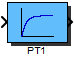
\includegraphics{PT1}\end{figure} 

\begin{XtoCtabular}{Inports}
In & Input In(k)\tabularnewline
\hline
\end{XtoCtabular}


\begin{XtoCtabular}{Outports}
Out & Output Out(k)\tabularnewline
\hline
\end{XtoCtabular}

\begin{XtoCtabular}{Mask Parameters}
V & Gain\tabularnewline
\hline
fc & Cut off frequency of low pass filter\tabularnewline
\hline
ts\_fact & Multiplication factor of base sampling time (in integer format)\tabularnewline
\hline
method & Discretization method\tabularnewline
\hline
\end{XtoCtabular}

\subsubsection*{Description:}
First order low pass:

    G(s) = V/(s/w + 1)

% include optional documentation file
\InputIfFileExists{\XcHomePath/Library/Control/Doc/PT1_Info.tex}{\vspace{1ex}}{}

\subsubsection*{Implementations:}
\begin{tabular}{l l}
\textbf{FiP8} & 8 Bit Fixed Point Implementation\tabularnewline
\textbf{FiP16} & 16 Bit Fixed Point Implementation\tabularnewline
\textbf{FiP32} & 32 Bit Fixed Point Implementation\tabularnewline
\textbf{Float32} & 32 Bit Floating Point Implementation\tabularnewline
\textbf{Float64} & 64 Bit Floating Point Implementation\tabularnewline
\end{tabular}

\XtoCImplementation{FiP8}
\index{Block ID!3312}
\nopagebreak[0]
% Implementation details
\begin{tabular}{l l}
\textbf{Name} & FiP8 \tabularnewline
\textbf{ID} & 3312 \tabularnewline
\textbf{Revision} & 0.1 \tabularnewline
\textbf{C filename} & PT1\_FiP8.c \tabularnewline
\textbf{H filename} & PT1\_FiP8.h \tabularnewline
\end{tabular}
\vspace{1ex}

8 Bit Fixed Point Implementation

\begin{XtoCtabular}{Controller Parameters}
b0 & \tabularnewline
\hline
b1 & \tabularnewline
\hline
a0 & \tabularnewline
\hline
sfrb & \tabularnewline
\hline
sfra & \tabularnewline
\hline
in\_old & In(k-1)\tabularnewline
\hline
\end{XtoCtabular}

% Implementation data structure
\XtoCDataStruct{Data Structure:}
\begin{lstlisting}
typedef struct {
     uint16        ID;
     int8          *In;
     int8          Out;
     int8          b0;
     int8          b1;
     int8          a0;
     int8          sfrb;
     int8          sfra;
     int8          in_old;
} PT1_FIP8;
\end{lstlisting}

\ifdefined \AddTestReports
\InputIfFileExists{\XcHomePath/Library/Control/Doc/Test_PT1_FiP8.tex}{}{}
\fi
\XtoCImplementation{FiP16}
\index{Block ID!3313}
\nopagebreak[0]
% Implementation details
\begin{tabular}{l l}
\textbf{Name} & FiP16 \tabularnewline
\textbf{ID} & 3313 \tabularnewline
\textbf{Revision} & 0.1 \tabularnewline
\textbf{C filename} & PT1\_FiP16.c \tabularnewline
\textbf{H filename} & PT1\_FiP16.h \tabularnewline
\end{tabular}
\vspace{1ex}

16 Bit Fixed Point Implementation

\begin{XtoCtabular}{Controller Parameters}
b0 & \tabularnewline
\hline
b1 & \tabularnewline
\hline
a0 & \tabularnewline
\hline
sfrb & \tabularnewline
\hline
sfra & \tabularnewline
\hline
in\_old & In(k-1)\tabularnewline
\hline
\end{XtoCtabular}

% Implementation data structure
\XtoCDataStruct{Data Structure:}
\begin{lstlisting}
typedef struct {
     uint16        ID;
     int16         *In;
     int16         Out;
     int16         b0;
     int16         b1;
     int16         a0;
     int8          sfrb;
     int8          sfra;
     int16         in_old;
} PT1_FIP16;
\end{lstlisting}

\ifdefined \AddTestReports
\InputIfFileExists{\XcHomePath/Library/Control/Doc/Test_PT1_FiP16.tex}{}{}
\fi
\XtoCImplementation{FiP32}
\index{Block ID!3314}
\nopagebreak[0]
% Implementation details
\begin{tabular}{l l}
\textbf{Name} & FiP32 \tabularnewline
\textbf{ID} & 3314 \tabularnewline
\textbf{Revision} & 0.1 \tabularnewline
\textbf{C filename} & PT1\_FiP32.c \tabularnewline
\textbf{H filename} & PT1\_FiP32.h \tabularnewline
\end{tabular}
\vspace{1ex}

32 Bit Fixed Point Implementation

\begin{XtoCtabular}{Controller Parameters}
b0 & \tabularnewline
\hline
b1 & \tabularnewline
\hline
a0 & \tabularnewline
\hline
sfrb & \tabularnewline
\hline
sfra & \tabularnewline
\hline
in\_old & In(k-1)\tabularnewline
\hline
\end{XtoCtabular}

% Implementation data structure
\XtoCDataStruct{Data Structure:}
\begin{lstlisting}
typedef struct {
     uint16        ID;
     int32         *In;
     int32         Out;
     int32         b0;
     int32         b1;
     int32         a0;
     int8          sfrb;
     int8          sfra;
     int32         in_old;
} PT1_FIP32;
\end{lstlisting}

\ifdefined \AddTestReports
\InputIfFileExists{\XcHomePath/Library/Control/Doc/Test_PT1_FiP32.tex}{}{}
\fi
\XtoCImplementation{Float32}
\index{Block ID!3315}
\nopagebreak[0]
% Implementation details
\begin{tabular}{l l}
\textbf{Name} & Float32 \tabularnewline
\textbf{ID} & 3315 \tabularnewline
\textbf{Revision} & 0.1 \tabularnewline
\textbf{C filename} & PT1\_Float32.c \tabularnewline
\textbf{H filename} & PT1\_Float32.h \tabularnewline
\end{tabular}
\vspace{1ex}

32 Bit Floating Point Implementation

\begin{XtoCtabular}{Controller Parameters}
b0 & Coefficient b0\tabularnewline
\hline
b1 & Coefficient b1\tabularnewline
\hline
a0 & Coefficient a0\tabularnewline
\hline
in\_old & In(k-1)\tabularnewline
\hline
\end{XtoCtabular}

% Implementation data structure
\XtoCDataStruct{Data Structure:}
\begin{lstlisting}
typedef struct {
     uint16        ID;
     float32       *In;
     float32       Out;
     float32       b0;
     float32       b1;
     float32       a0;
     float32       in_old;
} PT1_FLOAT32;
\end{lstlisting}

\ifdefined \AddTestReports
\InputIfFileExists{\XcHomePath/Library/Control/Doc/Test_PT1_Float32.tex}{}{}
\fi
\XtoCImplementation{Float64}
\index{Block ID!3316}
\nopagebreak[0]
% Implementation details
\begin{tabular}{l l}
\textbf{Name} & Float64 \tabularnewline
\textbf{ID} & 3316 \tabularnewline
\textbf{Revision} & 0.1 \tabularnewline
\textbf{C filename} & PT1\_Float64.c \tabularnewline
\textbf{H filename} & PT1\_Float64.h \tabularnewline
\end{tabular}
\vspace{1ex}

64 Bit Floating Point Implementation

\begin{XtoCtabular}{Controller Parameters}
b0 & Coefficient b0\tabularnewline
\hline
b1 & Coefficient b1\tabularnewline
\hline
a0 & Coefficient a0\tabularnewline
\hline
in\_old & In(k-1)\tabularnewline
\hline
\end{XtoCtabular}

% Implementation data structure
\XtoCDataStruct{Data Structure:}
\begin{lstlisting}
typedef struct {
     uint16        ID;
     float64       *In;
     float64       Out;
     float64       b0;
     float64       b1;
     float64       a0;
     float64       in_old;
} PT1_FLOAT64;
\end{lstlisting}

\ifdefined \AddTestReports
\InputIfFileExists{\XcHomePath/Library/Control/Doc/Test_PT1_Float64.tex}{}{}
\fi
